% chapter5.tex -- What the Paper Did and Why It Cannot Be Used for Biconnected Graphs
% Based on the author's UGThesis.docx.

\chapter{What the Paper Did and Why It Cannot Be Used for Biconnected Graphs}
\label{ch:paper_limitation}

In this chapter we describe the algorithm of Parvez, Rahman, and Nakano~\cite{parvez2011} for generating all triangulations of a triconnected plane graph. 
We then explain why this algorithm fails when applied directly to biconnected graphs, focusing on the multi-edge problem caused by separation pairs.

\section{The Parvez–Rahman–Nakano Algorithm for Triconnected Graphs}
\label{sec:paper_triconnected}

The algorithm for triconnected plane graphs follows the same high-level structure as the cycle algorithm presented in Chapter~\ref{ch:cycle_algorithm}, but now multiple faces are processed simultaneously. 
Given a triconnected plane graph \(G\) with \(n\) vertices and \(k\) faces \(F_1, F_2, \dots, F_k\), the algorithm constructs a \emph{global genealogical tree} \(\mathcal{T}(G)\) of triangulations of \(G\).

\subsection{Building the Root Triangulation}
\label{subsec:paper_root}

For each face \(F_i\) (a cycle), we choose a root vertex arbitrarily and construct the fan triangulation for that face. 
The root triangulation \(T_R\) of \(G\) is obtained by taking the union of these face triangulations. 
Since \(G\) is triconnected, the faces are independent: adding chords in one face does not affect the other faces.

\begin{figure}[htbp]
    \centering
    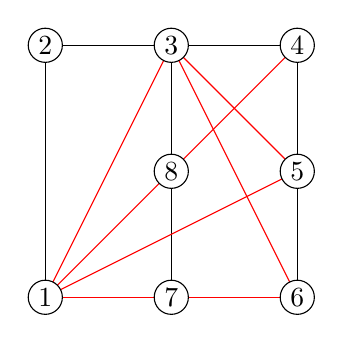
\begin{tikzpicture}[scale=0.8, every node/.style={circle, draw, fill=white, inner sep=1.5pt}]
        % A triconnected plane graph (triangulated outer face, inner face)
        \coordinate (v1) at (0,2);
        \coordinate (v2) at (0,6);
        \coordinate (v3) at (2,6);
        \coordinate (v4) at (4,6);
        \coordinate (v5) at (4,4);
        \coordinate (v6) at (4,2);
        \coordinate (v7) at (2,2);
        \coordinate (v8) at (2,4);
        \draw (v1)--(v2)--(v3)--(v4)--(v5)--(v6)--(v7)--(v8);
        \draw (v1)--(v7);
        \draw (v3)--(v8);
        \draw[red] (v1)--(v3);
        \draw[red] (v1)--(v4);
        \draw[red] (v1)--(v5);
        \draw[red] (v1)--(v6);
        \draw[red] (v3)--(v5);
        \draw[red] (v3)--(v6);
        \node at (v1) {1};
        \node at (v2) {2};
        \node at (v3) {3};
        \node at (v4) {4};
        \node at (v5) {5};
        \node at (v6) {6};
        \node at (v7) {7};
        \node at (v8) {8};
    \end{tikzpicture}
    \caption{A root triangulation of a triconnected plane graph. The root vertex for each face is chosen independently; all chords are added simultaneously.}
    \label{fig:paper_root}
\end{figure}

The generating set \(GS^0\) of the root triangulation is the union of the generating sets of the individual faces. 
Since each face with \(n_i\) vertices contributes \(n_i - 3\) generating chords, the total number of generating chords in the root is \(\sum_i (n_i - 3) = O(n)\) (by Euler’s formula).

\subsection{Generating Child Triangulations}
\label{subsec:paper_child}

From a triangulation \(T\) of \(G\), a child triangulation \(T'\) is generated by flipping a generating chord in one eligible face. 
A face \(F_i\) is called \textbf{eligible} if all faces with smaller indices have already been processed; the algorithm processes faces in a fixed order.

The key property that enables constant-time generation is that flipping a generating chord in a face affects only that face. 
Because the graph is triconnected, the flipped chord cannot create a multi-edge with chords from other faces. 
Therefore, the algorithm can simply flip any generating chord and obtain a new valid triangulation.

\subsection{Time and Space Complexity}
\label{subsec:paper_complexity}

The depth of the global genealogical tree is bounded by the total number of generating chords, which is \(O(n)\). 
Each flip operation takes \(O(1)\) time (updating the chord lists and opposite pairs for the affected face). 
Hence the algorithm generates all triangulations of \(G\) in \(O(1)\) amortised time per triangulation, using \(O(n)\) space.

\section{Why the Algorithm Cannot Be Used for Biconnected Graphs}
\label{sec:paper_failure}

The authors of the original paper explicitly limited their algorithm to triconnected plane graphs. 
The reason is that in biconnected graphs, separation pairs can exist, and these cause a fundamental problem: the \textbf{multi-edge problem}.

\subsection{Separation Pairs in Biconnected Graphs}
\label{subsec:separation_pairs}

Recall from Chapter~\ref{ch:preliminaries} that a separation pair is a pair of vertices whose removal disconnects the graph. 
Biconnected graphs may contain separation pairs, while triconnected graphs do not.

\begin{figure}[htbp]
    \centering
    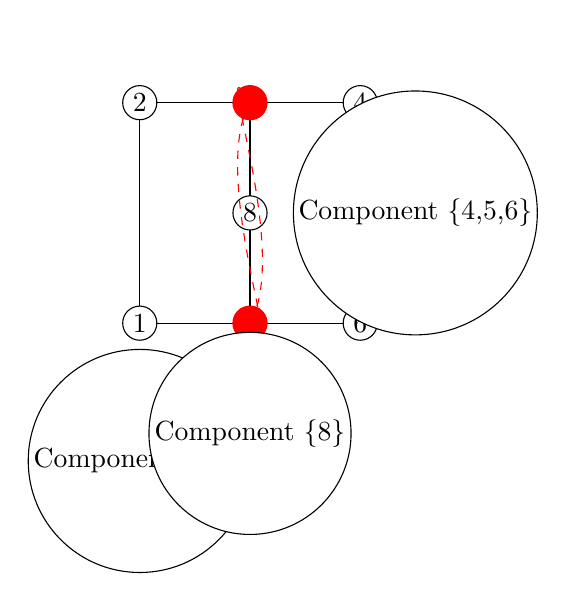
\begin{tikzpicture}[scale=0.7, every node/.style={circle, draw, fill=white, inner sep=1.5pt}]
        \coordinate (v1) at (0,2);
        \coordinate (v2) at (0,6);
        \coordinate (v3) at (2,6);
        \coordinate (v4) at (4,6);
        \coordinate (v5) at (4,4);
        \coordinate (v6) at (4,2);
        \coordinate (v7) at (2,2);
        \coordinate (v8) at (2,4);
        \draw (v1)--(v2)--(v3)--(v4)--(v5)--(v6)--(v7)--(v8);
        \draw (v1)--(v7);
        \draw (v3)--(v8);
        \node at (v1) {1};
        \node at (v2) {2};
        \node[red] at (v3) {3};
        \node at (v4) {4};
        \node at (v5) {5};
        \node at (v6) {6};
        \node[red] at (v7) {7};
        \node at (v8) {8};
        % Indicate components after removal
        \draw[red, dashed] (v3) to[out=120,in=60] (v7);
        \draw[red, dashed] (v3) to[out=-120,in=-60] (v7);
        \node at (0, -0.5) {Component \{1,2\}};
        \node at (5, 4) {Component \{4,5,6\}};
        \node at (2, 0) {Component \{8\}};
    \end{tikzpicture}
    \caption{A biconnected plane graph with separation pair \((3,7)\). Removing vertices 3 and 7 leaves three components: \(\{1,2\}\), \(\{4,5,6\}\), and \(\{8\}\).}
    \label{fig:paper_separation_pair}
\end{figure}

\subsection{The Multi-Edge Problem}
\label{subsec:multiedge_problem}

In a triconnected graph, the triangulation of different faces are independent: any chord added in one face cannot appear in another face because that would require the two faces to share a common chord, which would create a separation pair. 
In a biconnected graph with a separation pair \((a,b)\), however, there exist two faces (one on each side of the separation pair) that share the same boundary vertices \(a\) and \(b\).

\begin{figure}[htbp]
    \centering
    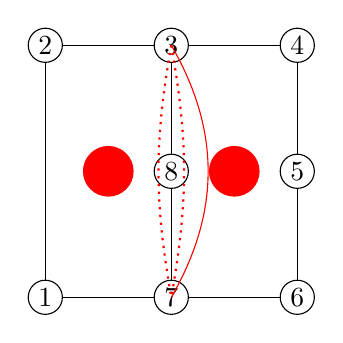
\begin{tikzpicture}[scale=0.8, every node/.style={circle, draw, fill=white, inner sep=1.5pt}]
        \coordinate (v1) at (0,2);
        \coordinate (v2) at (0,6);
        \coordinate (v3) at (2,6);
        \coordinate (v4) at (4,6);
        \coordinate (v5) at (4,4);
        \coordinate (v6) at (4,2);
        \coordinate (v7) at (2,2);
        \coordinate (v8) at (2,4);
        \draw (v1)--(v2)--(v3)--(v4)--(v5)--(v6)--(v7)--(v8);
        \draw (v1)--(v7);
        \draw (v3)--(v8);
        \node at (v1) {1};
        \node at (v2) {2};
        \node at (v3) {3};
        \node at (v4) {4};
        \node at (v5) {5};
        \node at (v6) {6};
        \node at (v7) {7};
        \node at (v8) {8};
        \node[red] at (1,4) {\(F_1\)};
        \node[red] at (3,4) {\(F_2\)};
        \draw[red, dotted, thick] (v3) to[out=-100,in=100] (v7);
        \draw[red, dotted, thick] (v3) to[out=-80,in=80] (v7);
        \draw[red] (v3) to[out=-60,in=60] (v7);
    \end{tikzpicture}
    \caption{The separation pair \((3,7)\) appears on two faces \(F_1\) and \(F_2\). Triangulating each face independently may add the same chord \((3,7)\) twice, creating a multi-edge.}
    \label{fig:paper_multiedge}
\end{figure}

If we independently triangulate the two faces using the algorithm of Parvez et al., it is possible that both faces receive the chord \((a,b)\) (the chord that directly connects the separation pair). 
In a simple graph, having two copies of the same edge is not allowed. 
Thus the resulting structure would contain a multi-edge, which is not a valid triangulation of a simple graph.

\subsection{Why the Original Algorithm Fails}
\label{subsec:original_fails}

The original algorithm was designed assuming that no multi-edge can appear. 
It processes all faces in parallel, flipping chords without checking whether the new chord already exists in another face. 
In a triconnected graph this assumption holds, but in a biconnected graph it does not. 
Therefore a direct application of the algorithm to a biconnected graph would generate many invalid triangulations containing multi-edges.

Moreover, simply discarding invalid triangulations is not sufficient because:
\begin{enumerate}
    \item Checking for multi-edges would require additional time per flip, breaking the \(O(1)\) amortised guarantee.
    \item The number of invalid triangulations could be large, wasting substantial computational resources.
    \item More importantly, the genealogical tree structure would be corrupted: a child might have a valid parent, but its descendants could all be invalid due to a persistent multi-edge. Pruning such branches requires careful analysis.
\end{enumerate}

\section{Conclusion}
\label{sec:paper_conclusion}

The Parvez-Rahman-Nakano algorithm is optimal for triconnected plane graphs but cannot be used directly for biconnected graphs because of the multi-edge problem caused by separation pairs. 
In the following chapters we develop a new approach that processes faces sequentially, uses a global chord set to detect conflicts, and prunes invalid branches safely, thereby extending the optimal complexity to biconnected graphs.